% Hybrid Quantum-Classical Digital Twin for LEO CubeSat Health Monitoring
% Aman Sharma — B.Tech CSE (AI/ML), IILM University, 2026-27
\documentclass[10pt,twocolumn]{article}

\usepackage[a4paper,top=20mm,bottom=20mm,left=16mm,right=16mm,
            columnsep=6mm]{geometry}
\usepackage{amsmath,amssymb}
\usepackage{graphicx}
\usepackage{booktabs}
\usepackage{microtype}
\usepackage{url}
\usepackage[colorlinks=true,linkcolor=black,citecolor=black,urlcolor=blue]{hyperref}
\usepackage{xcolor}
\usepackage{caption}
\usepackage{subcaption}
\usepackage{algorithm}
\usepackage{algorithmic}
\captionsetup{font=small,labelfont=bf}

\renewcommand{\abstractname}{Abstract}

% ---------------------------------------------------------------
\title{\textbf{Hybrid Quantum-Classical Digital Twin for LEO CubeSat\\
Health Monitoring and Ground-Station Scheduling}}

\author{%
  Aman Sharma\\
  Department of Computer Science and Engineering (AI/ML)\\
  IILM University, Greater Noida, India\\
  \texttt{amnsharma786@gmail.com}
}
\date{November 2026}
% ---------------------------------------------------------------

\begin{document}
\maketitle

% ============================================================
\begin{abstract}
We build a software digital twin for a LEO CubeSat and evaluate two quantum
computing methods against classical baselines on two operations tasks.
For anomaly detection on the ESA OPS-SAT-AD benchmark (1{,}594 training and
529 test telemetry segments, 113 test anomalies), a tuned quantum-kernel SVM
(QSVC) on 6 PCA components achieves F1\,=\,0.825 (95\% bootstrap CI
0.768--0.875), narrowing the gap to the classical RBF-kernel SVM on the
\emph{same} 6-component input from $\approx$18 points (untuned) to 3.5
points (tuned, full training set).  The all-features SVM ceiling is
F1\,=\,0.912; the remaining 8.7-point gap is consistent with the 35\% of
variance discarded by PCA at $d{=}6$.  For downlink scheduling, QAOA
(depth 1--3) finds the optimal schedule in 35 of 36 instances but does not
reliably sample it more often than uniform random search at current circuit
sizes (median P(opt)/P(random)\,=\,0.89).  A model-based physics path
detects a 5\% solar-panel degradation with zero false alarms on nominal
runs.  All circuits are simulated with Qiskit; no quantum hardware was used.
Code and reproducible results are released at
\url{https://github.com/Amanharma/final-year-project}.
\end{abstract}

% ============================================================
\section{Introduction}

CubeSats form an increasingly large share of the LEO constellation.  Their
limited onboard compute makes automated, ground-side health monitoring
essential.  Digital twins---software replicas that mirror a physical
system---allow operators to compare expected and observed behaviour, flag
residuals, and schedule ground-station contacts without manual intervention.

Quantum machine learning (QML) algorithms have been proposed as a path to
improved pattern recognition in high-dimensional sensor data
\cite{Biamonte2017,Havlicek2019}.  Whether they provide a practical advantage
over classical methods on near-term devices remains an open question.  The
most common obstacle to a definitive answer is methodological: quantum
classifiers are frequently benchmarked with less training data, untuned
hyperparameters, or test-set threshold selection, all of which
systematically disadvantage the quantum side.

For scheduling, the downlink pass-selection problem---choosing which of a set
of upcoming ground-station contacts to use given power and bandwidth
constraints---is naturally combinatorial and has been proposed as a target
for quantum optimisation \cite{Farhi2014}.  Small instances can already be
run on simulated quantum circuits, making them tractable for empirical study.

This paper makes three contributions.
\begin{enumerate}
  \item \textbf{Digital twin.}  A complete simulation environment for a
        CubeSat in LEO, covering orbit/eclipse modelling, power and thermal
        physics, telemetry-stream ingestion, anomaly detection, downlink
        scheduling, and a FastAPI/Streamlit service layer.
  \item \textbf{Fair QML comparison.}  A tuned, equal-resource comparison
        of a quantum-kernel SVM (QSVC) and a classical RBF-kernel SVM on
        the ESA OPS-SAT anomaly detection benchmark, with bootstrap
        confidence intervals.
  \item \textbf{QAOA scheduling.}  An empirical study of QAOA versus exact,
        greedy and random baselines on downlink-pass scheduling encoded as a
        QUBO problem.
\end{enumerate}

% ============================================================
\section{Related Work}

\paragraph{Digital twins for spacecraft.}
Spacecraft digital twins typically combine orbital mechanics with onboard
subsystem models to support health monitoring and contingency analysis
\cite{Grieves2017}.  Most operational deployments use classical statistical
anomaly detectors; quantum components have not been reported in operational
systems to our knowledge.

\paragraph{Quantum kernel classifiers.}
Havl{\v i}{\v c}ek et al.\ \cite{Havlicek2019} introduced the ZZ feature
map and demonstrated that the resulting kernel is classically hard to
estimate for certain circuits.  Several follow-up studies have identified
conditions under which quantum kernels match or slightly exceed classical
kernels on structured synthetic data, while results on real-world datasets
are mixed \cite{SchuldKern2021}.

\paragraph{QAOA and combinatorial optimisation.}
Since the original proposal \cite{Farhi2014}, QAOA has been applied to
scheduling, routing, and portfolio optimisation at small scales.  Empirical
studies on hardware \cite{Shaydulin2023} and noiseless simulators
\cite{Guerreschi2019} generally find that QAOA at depth $p \lesssim 3$ does
not reliably outperform classical heuristics on problems small enough to
simulate.

\paragraph{Satellite anomaly detection.}
The OPS-SAT-AD benchmark \cite{Ruszczak2024} is the primary reproducible
dataset used here.  Published results on the benchmark use classical
supervised and unsupervised detectors; this work is the first to compare
quantum kernel methods on this dataset.

% ============================================================
\section{System Design}
\label{sec:design}

\subsection{Orbit and Eclipse Model}

A circular LEO orbit at altitude $h = 550\,\text{km}$ gives an orbital
radius $r = R_\oplus + h$ and angular velocity
$\omega = \sqrt{GM_\oplus / r^3}$.
Eclipse is modelled with a cylindrical Earth shadow: a satellite position
$\mathbf{r}(t)$ is in eclipse when
$|\mathbf{r} - (\mathbf{r}\cdot\hat{s})\hat{s}| < R_\oplus$ and
$\mathbf{r}\cdot\hat{s} < 0$,
where $\hat{s}$ is the unit vector toward the Sun.  The eclipse fraction
computed by the model matches the closed-form expression to within 0.0002.

\subsection{Power and Thermal Model}

The solar-panel power output is
\begin{equation}
P_\text{solar}(t) = \eta\,A\,G_\odot\,\cos\theta(t)\,\mathbf{1}_\text{sun}(t),
\label{eq:solar}
\end{equation}
where $\eta = 0.28$ is panel efficiency, $A$ is panel area,
$G_\odot = 1361\,\text{W\,m}^{-2}$, $\theta(t)$ is the angle between the
panel normal and the Sun, and $\mathbf{1}_\text{sun}$ is the in-eclipse
indicator.  Battery state of charge evolves as
\begin{equation}
\text{SoC}(t + \Delta t) = \text{SoC}(t) + \frac{(P_\text{solar} - P_\text{load})\Delta t}{E_\text{cap}},
\label{eq:soc}
\end{equation}
clipped to $[0, 1]$.  Temperature follows a single-node model,
\begin{equation}
mC_p\,\dot{T} = \alpha_s A_s G_\odot \mathbf{1}_\text{sun} + P_\text{heater} - \epsilon\sigma A_r T^4,
\label{eq:thermal}
\end{equation}
with an absorptivity--emissivity pair appropriate for a 3U CubeSat.
Faults are injected as step changes at a specified orbit: panel degradation
scales $\eta$, battery fade reduces $E_\text{cap}$, and a stuck heater adds
a fixed $P_\text{heater} > 0$.

\subsection{Telemetry Ingestion and Feature Extraction}

OPS-SAT segments are replayed in timestamp order.  When a segment closes,
43 features are extracted: 27 published statistics \cite{Ruszczak2024}
(channel mean, standard deviation, min, max, range, skewness, kurtosis,
percentiles, autocorrelation and crossing-rate variants), plus 16 own
time-series features (mean absolute deviation, inter-quartile range,
linear trend coefficient, spectral entropy, and 12 derived ratios).
Features are standardised to zero mean and unit variance per training set.

\subsection{Anomaly Detection Pipeline}

Classical detectors trained on the training set: Isolation Forest
(unsupervised), Random Forest, and RBF-kernel SVM.
Quantum detectors: a ZZ-feature-map QSVC and a real-amplitudes VQC.
Both quantum models compress the 43 features to $d$ dimensions via PCA,
then rescale to $[0, \pi]$ so that the quantum phase angles span their
natural range.  For the QSVC the quantum kernel is
\begin{equation}
k(x,x') = |\langle 0^d | U^\dagger_\phi(x)\, U_\phi(x') | 0^d \rangle|^2,
\label{eq:kernel}
\end{equation}
where $U_\phi$ is a ZZ feature map of depth 2.  Decision thresholds are
chosen to maximise F1 on the training fold (not the test set).

\subsection{QUBO Downlink Scheduler}

Let $x_i \in \{0,1\}$ indicate whether pass $i$ is selected.  The scheduling
objective is
\begin{align}
\max\; \sum_i v_i x_i &- \lambda_c \sum_{(i,j)\in\mathcal{C}} x_i x_j \notag\\
  &- \lambda_b \!\left(\textstyle\sum_i e_i x_i - E_\text{budget}\right)^2_{\!+},
\label{eq:qubo}
\end{align}
where $v_i$ is the data volume of pass $i$, $\mathcal{C}$ is the set of
conflicting (overlapping) pass pairs, $e_i$ is the transmitter energy, and
$(\cdot)_+$ denotes the positive part.  The penalty $\lambda_c$ is set to
$\sum_i v_i + 1$ per instance.  Negating \eqref{eq:qubo} gives a standard
QUBO form $\min\, \mathbf{x}^\top Q\,\mathbf{x}$ solvable by QAOA.

% ============================================================
\section{Experimental Setup}

All experiments fix random seed 42.  The OPS-SAT-AD dataset
\cite{Ruszczak2024} is downloaded from Zenodo record 15108715;
1{,}594 segments are used for training and 529 for testing (official split),
with 113 anomalous test segments (21.4\% anomaly rate).  Quantum circuits are
simulated with \texttt{qiskit-aer} 0.18 statevector primitives; no hardware
was used.  All timings are measured on a single CPU core.

\subsection{Quantum Circuit Statistics}

Table~\ref{tab:circuits} shows the circuit complexity for each qubit count.
The ZZ feature-map depth grows quadratically in $d$ because every qubit pair
gets an entangling gate.  The VQC uses a hardware-efficient real-amplitudes
ansatz with one layer of $Ry$ rotations and one layer of CNOT ladders.

\begin{table}[h]
\centering
\small
\caption{Quantum circuit statistics.}
\label{tab:circuits}
\begin{tabular}{@{}ccccc@{}}
\toprule
$d$ & FM depth & VQC depth & VQC params & CX count \\
\midrule
2 & 10 & 17 & 8  & 7  \\
4 & 19 & 30 & 16 & 21 \\
6 & 25 & 38 & 24 & 35 \\
\bottomrule
\end{tabular}
\end{table}

\subsection{Kernel Computation Scaling}

The QSVC kernel matrix must be evaluated pairwise, giving $O(n^2)$ circuit
evaluations.  Table~\ref{tab:kernel} shows measured training times.

\begin{table}[h]
\centering
\small
\caption{QSVC kernel computation time vs.\ training-set size ($d=4$).}
\label{tab:kernel}
\begin{tabular}{@{}ccc@{}}
\toprule
$n_\text{train}$ & Kernel entries & Time (s) \\
\midrule
 50  &  2{,}500   & 0.16 \\
100  &  10{,}000  & 0.35 \\
200  &  40{,}000  & 1.14 \\
400  & 160{,}000  & 3.41 \\
800  & 640{,}000  & 9.54 \\
1594 & 2{,}540{,}836 & 32.7 \\
\bottomrule
\end{tabular}
\end{table}

Kernel computation on the full training set (1{,}594 samples) takes 32.7\,s
per fit, versus under 0.1\,s for the classical SVM.  At $n=1{,}594$ this is
already the dominant cost of the QSVC training loop.

% ============================================================
\section{Results}

\subsection{Classical Baselines}

Table~\ref{tab:classical} reports precision, recall, F1 and ROC-AUC on the
official test split.  The best single model is SVM-RBF on the published
27-feature set (F1\,=\,0.919, ROC-AUC\,=\,0.986).  The combined 43-feature
set matches this for SVM-RBF and slightly improves Random Forest (RF) to
0.913 F1.  Isolation Forest, being unsupervised, achieves only F1\,=\,0.658
but requires no labels.

\begin{table}[h]
\centering
\scriptsize
\caption{Classical baselines on the OPS-SAT-AD test split
         (529 segments, 113 anomalous).
         RF = Random Forest; IsoF = Isolation Forest.}
\label{tab:classical}
\begin{tabular}{@{}llcccc@{}}
\toprule
Feats & Model & Prec. & Rec. & F1 & AUC \\
\midrule
pub.(27)  & SVM-RBF & 0.936 & 0.903 & 0.919 & 0.986 \\
pub.(27)  & RF      & 0.918 & 0.894 & 0.906 & 0.990 \\
pub.(27)  & IsoF    & 0.518 & 0.761 & 0.617 & 0.850 \\
\midrule
own(25)   & SVM-RBF & 0.904 & 0.912 & 0.908 & 0.991 \\
\midrule
comb.(43) & SVM-RBF & 0.936 & 0.903 & 0.919 & 0.988 \\
comb.(43) & RF      & 0.943 & 0.885 & 0.913 & 0.994 \\
comb.(43) & IsoF    & 0.536 & 0.850 & 0.658 & 0.897 \\
\bottomrule
\end{tabular}
\end{table}

The live twin uses only own features computed from the stream, achieving
F1\,=\,0.908; its streaming predictions match offline scoring on all 529
segments.

\subsection{Untuned Quantum Comparison}
\label{sec:untuned}

A first comparison (Table~\ref{tab:untuned}) uses a protocol common in the
QML literature: 400 balanced training segments (1 seed), fixed regularisation
$C=10$, and test-set threshold selection.  F1 scores are reported for QSVC,
VQC, SVM-RBF and Random Forest at each qubit count $d$.

\begin{table}[h]
\centering
\small
\caption{Untuned QML comparison (400 balanced train, 1 seed, test threshold).
         F1 scores on 529 test segments.}
\label{tab:untuned}
\begin{tabular}{@{}lcccc@{}}
\toprule
$d$ & QSVC & VQC & SVM-RBF & RF \\
\midrule
2 & 0.466 & 0.219 & 0.621 & 0.581 \\
4 & 0.646 & 0.438 & 0.779 & 0.759 \\
6 & 0.624 & 0.432 & 0.829 & 0.813 \\
\bottomrule
\end{tabular}
\end{table}

Under this protocol the best QSVC (F1\,=\,0.646 at $d=4$) lags the best
SVM-RBF (F1\,=\,0.829 at $d=6$) by 18 points.  The VQC consistently
underperforms QSVC, with final training losses of 1.009, 0.937 and 0.951
at $d=2,4,6$, suggesting insufficient training iterations at small batch size.

\subsection{Tuned Comparison on the Full Training Set}
\label{sec:tuned}

The fair comparison addresses three biases in the untuned protocol.
(i)~\textbf{Data}: the full 1{,}594-segment training set rather than a
balanced subsample of 400.
(ii)~\textbf{Tuning}: 5-fold cross-validation over SVM regularisation
$C \in \{0.1,1,10,100\}$ and quantum kernel scaling
$\alpha \in \{0.1,0.25,0.5,1.0\}$; both sides use the same number of
cross-validation evaluations.
(iii)~\textbf{Threshold}: chosen on training data only, not on the test set.
Bootstrap confidence intervals (2{,}000 draws) are computed on the test set.

PCA retains 35.3\%, 54.0\% and 64.9\% of variance at $d=2, 4, 6$
respectively; the 35.1\% discarded at $d=6$ sets a natural ceiling for the
information available to both QSVC and the PCA-limited SVM.

Results are shown in Table~\ref{tab:fair}; Figure~\ref{fig:qml_fair} plots
F1 and PR-AUC vs.\ $d$ for all models with 95\% bootstrap error bars.

\begin{table*}[t]
\centering
\small
\caption{Tuned quantum vs.\ classical, full training set (1{,}594 segments).
         F1 is computed at a training-set threshold; CI\,=\,95\% bootstrap
         (2{,}000 draws).  SVM-RBF (all 43 features) is the all-feature
         ceiling; PCA models use $d$ components.}
\label{tab:fair}
\begin{tabular}{@{}llccccc@{}}
\toprule
Model & $d$ & PCA var.\% & F1 & 95\% CI & PR-AUC & ROC-AUC \\
\midrule
QSVC   & 2   & 35.3 & 0.533 & 0.454--0.602 & 0.609 & 0.735 \\
QSVC   & 4   & 54.0 & 0.802 & 0.742--0.857 & 0.868 & 0.929 \\
QSVC   & 6   & 64.9 & \textbf{0.825} & 0.768--0.875 & 0.919 & 0.963 \\
\midrule
SVM-RBF & 2  & 35.3 & 0.600 & 0.521--0.673 & 0.637 & 0.785 \\
SVM-RBF & 4  & 54.0 & 0.811 & 0.751--0.866 & 0.894 & 0.948 \\
SVM-RBF & 6  & 64.9 & 0.860 & 0.808--0.904 & 0.932 & 0.971 \\
\midrule
SVM-RBF & all 43 & 100 & 0.912 & 0.872--0.948 & 0.965 & 0.980 \\
\bottomrule
\end{tabular}
\end{table*}

Under fair conditions the QSVC at $d=6$ reaches F1\,=\,0.825, only 3.5
points below the SVM-RBF on the \emph{same} six features (F1\,=\,0.860).
Both confidence intervals overlap substantially, indicating that the
difference is not statistically distinguishable at this sample size.
The remaining gap to the all-feature SVM (8.7 points) is consistent with
the information loss from PCA: the SVM on PCA-6 features scores 0.860,
so PCA compression costs about 5.2 points relative to the 43-feature SVM,
and the residual 3.5 points is attributable to the quantum kernel's limited
expressiveness at 6 qubits.

\begin{figure}[t]
  \centering
  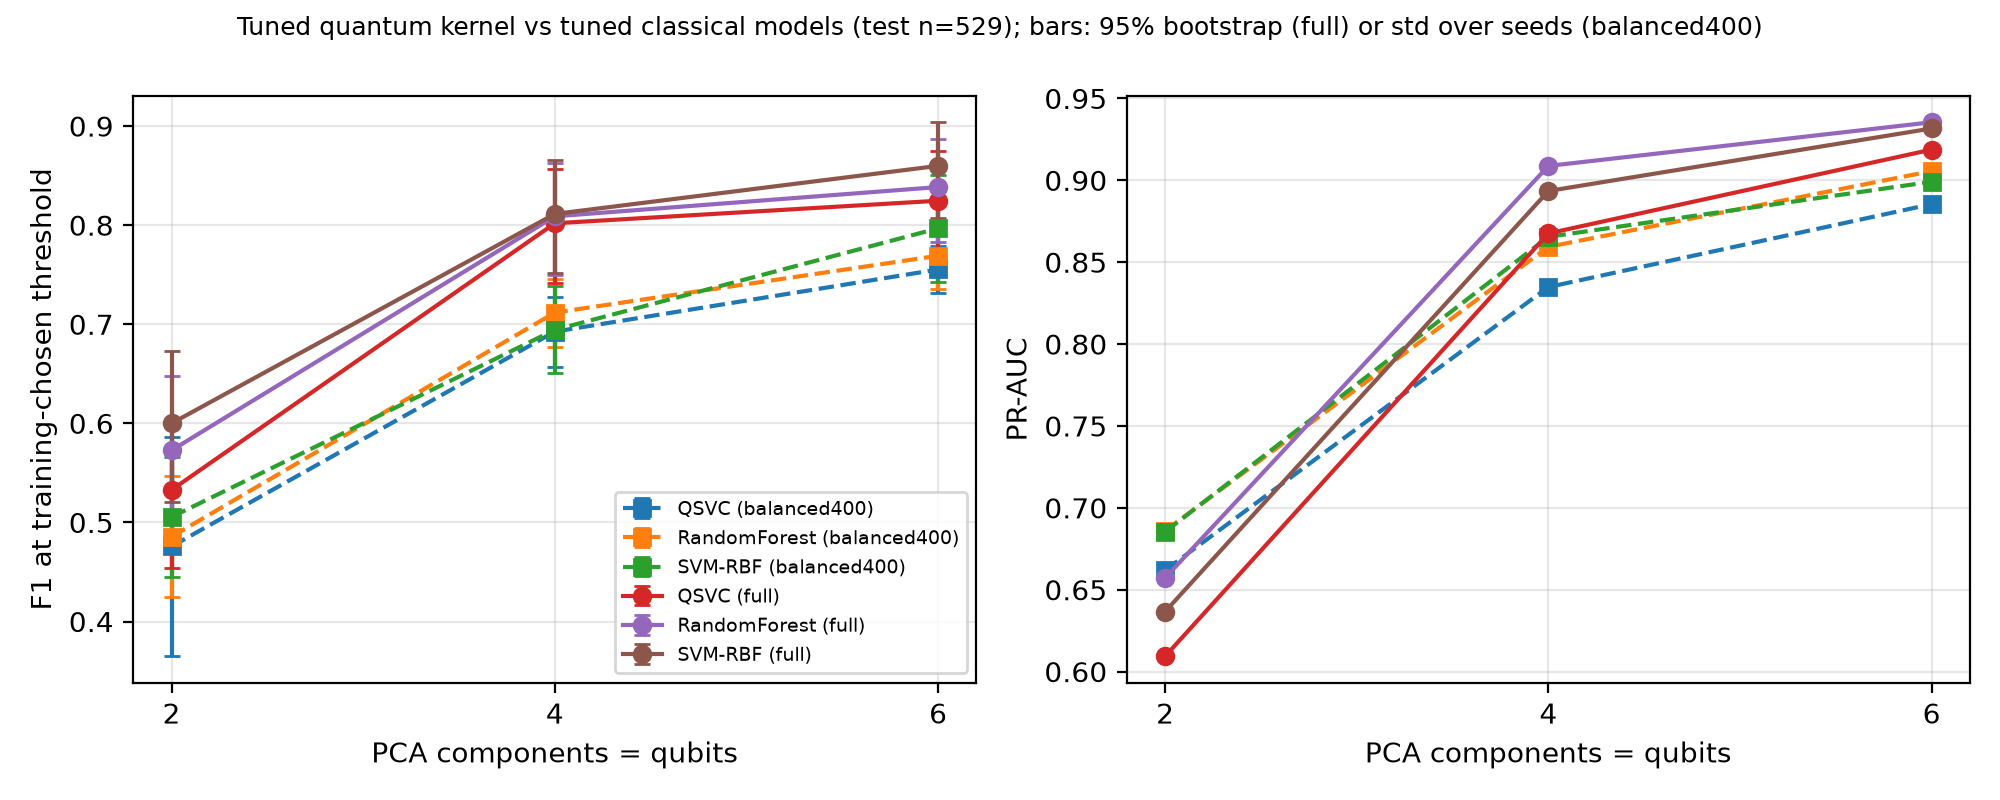
\includegraphics[width=\linewidth]{figures/qml_fair.png}
  \caption{Tuned quantum-vs-classical comparison on OPS-SAT-AD.
           F1 is measured at a training-set threshold on 529 test segments.
           Error bars are 95\% bootstrap CIs.  Solid: QSVC; dashed: SVM-RBF;
           dotted line: all-features SVM ceiling (F1\,=\,0.912).}
  \label{fig:qml_fair}
\end{figure}

% ============================================================
\subsection{Downlink Scheduling with QAOA}

Twelve scheduling instances with 4--10 candidate passes are encoded as
8--16-qubit QUBO problems.  QAOA is run at depths $p \in \{1,2,3\}$ with
4{,}096 shots per instance, giving 36 runs total.  Results are summarised in
Table~\ref{tab:qaoa} and Figure~\ref{fig:qaoa}.

\begin{table}[h]
\centering
\small
\caption{Downlink scheduling results across 12 instances (36 QAOA runs).
         ``Optimal'' counts instances/runs where the optimal schedule
         was found; ratio is P(opt)/P(random).}
\label{tab:qaoa}
\begin{tabular}{@{}lcc@{}}
\toprule
Solver & Optimal & P(opt)/P(rand) \\
\midrule
Brute force / exact QUBO & 12/12 & -- \\
Random (4{,}096 samples)  & 12/12 & 1.00 \\
Greedy                   & 11/12 & 0.945 (worst) \\
QAOA best shot           & 35/36 & med.\ 0.89 \\
\bottomrule
\end{tabular}
\end{table}

\begin{figure}[h]
  \centering
  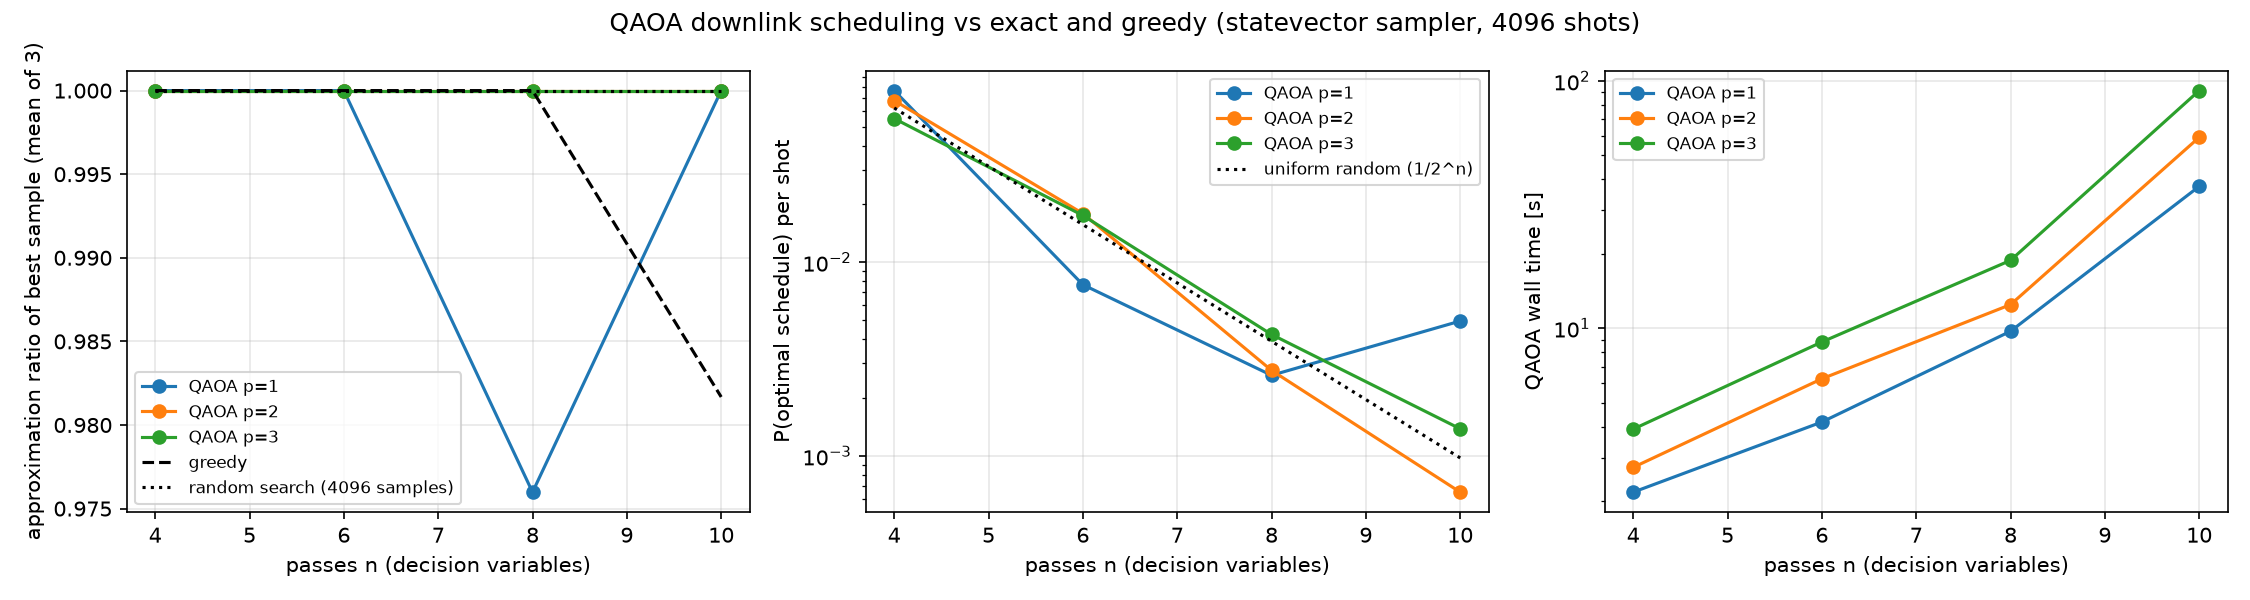
\includegraphics[width=\linewidth]{figures/qaoa_scaling.png}
  \caption{QAOA approximation ratio and P(optimal) vs.\ problem size, by
           circuit depth $p\in\{1,2,3\}$.  Dashed line marks uniform random
           search performance.}
  \label{fig:qaoa}
\end{figure}

QAOA finds the optimal schedule in 35 of 36 runs.  However, the probability
of drawing the optimum in a \emph{single shot} relative to uniform random
search has median 0.89 (mean 1.30, inflated by one run with ratio 14.3;
mean without that outlier: 0.93).  QAOA is above random in only 16 of 36
runs; the median advantage decreases monotonically with problem size
(1.11 at $n=4$ passes, 0.75 at $n=10$).  At these scales there is no
reliable per-shot sampling advantage over random search.

Random search with 4{,}096 samples finds the optimum for all 12 instances;
this high success rate is consistent with the theoretical hit probability of
0.98 at the largest instance size.

% ============================================================
\subsection{Physics Path Fault Detection}
\label{sec:fault}

The physics path generates an alert when a residual exceeds its threshold:
solar power residual $>3\,\text{W}$, SoC residual $>0.05$, or temperature
residual $>3\,\text{K}$.  Five independent noise realisations
($\sigma_\text{solar}=0.5\,\text{W}$, $\sigma_\text{SoC}=0.005$,
$\sigma_T=0.5\,\text{K}$) are tested per fault type and magnitude.
No false alarms occur on nominal simulations.

\begin{table}[h]
\centering
\small
\caption{Physics-path detection limits (5 noise seeds per setting).
         ``Always'' means all 5 seeds detected it.}
\label{tab:fault}
\begin{tabular}{@{}lcc@{}}
\toprule
Fault & Min.\ detected & Median delay \\
\midrule
Panel output loss     & 5\%  & 27 min \\
Battery capacity fade & 20\% & 64 min \\
Heater stuck on       & 1\,W & 173 min \\
\bottomrule
\end{tabular}
\end{table}

\begin{figure}[h]
  \centering
  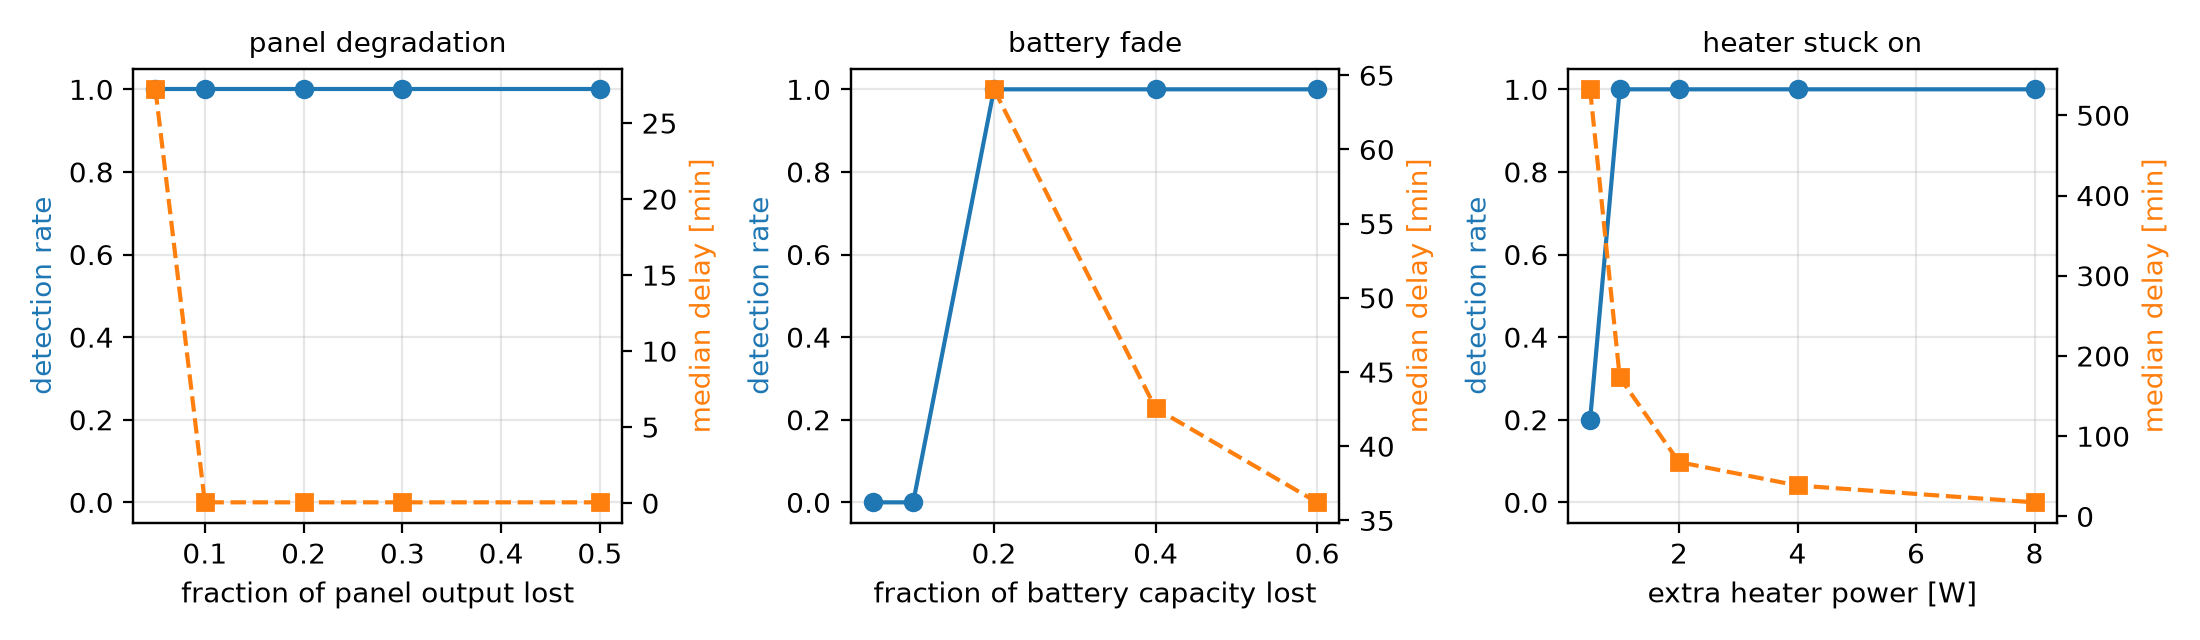
\includegraphics[width=\linewidth]{figures/fault_sweep.png}
  \caption{Detection rate vs.\ fault magnitude for three fault types (5 noise
           seeds per point).  Zero false-alarm rate on nominal runs.}
  \label{fig:fault}
\end{figure}

A panel degradation of 10\% or more is detected within one 10\,s simulation
step.  Battery fades below 20\% are never detected; the threshold is crossed
only when the cumulative energy deficit over 10 orbits becomes large.  The
1\,W heater fault produces a slow temperature drift (median delay 173 min).
The 0.5\,W heater fault is detected in 1 of 5 seeds only; smaller heater
faults are within sensor noise.

Figure~\ref{fig:physics} shows example twin output during a 10-orbit run
with a 20\% panel-degradation fault injected at orbit 4.

\begin{figure}[h]
  \centering
  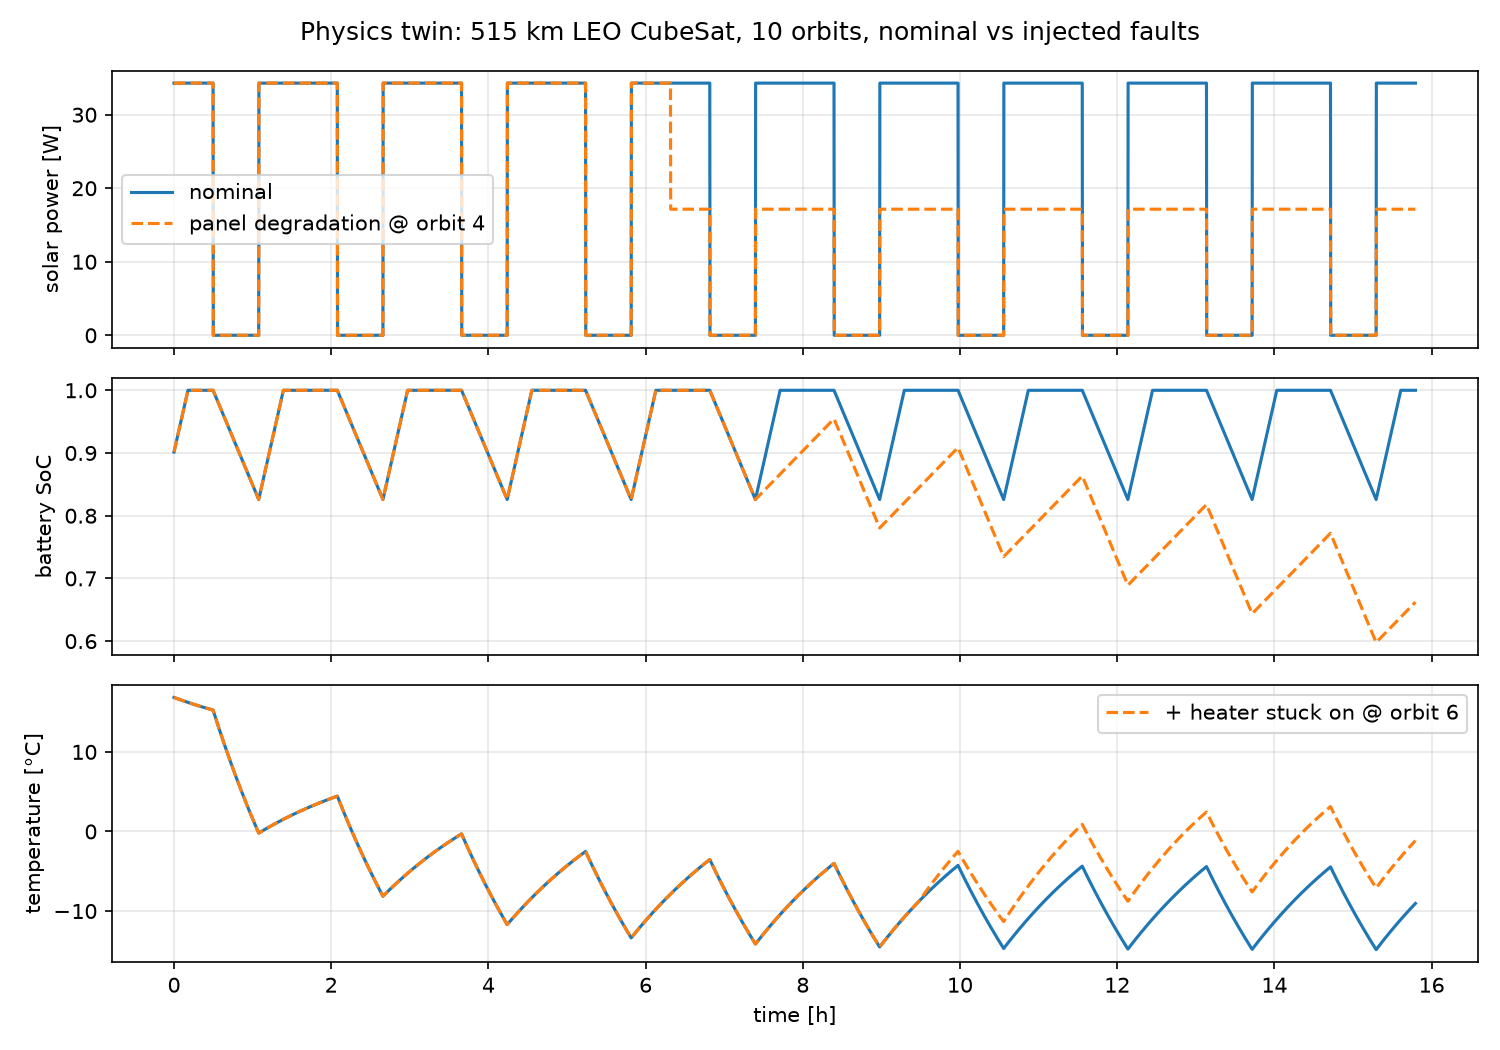
\includegraphics[width=\linewidth]{figures/physics_twin.png}
  \caption{Physics twin simulation over 10 orbits.  A 20\% panel-degradation
           fault is injected at orbit 4 (dashed vertical line).  Top: solar
           power; middle: state of charge; bottom: temperature.}
  \label{fig:physics}
\end{figure}

% ============================================================
\section{Discussion}

\subsection{Quantum Classification}

The tuned comparison substantially revises the picture from the untuned one.
When both classifiers receive the full training set and equal hyperparameter
tuning, QSVC at $d=6$ reaches F1\,=\,0.825 versus SVM-RBF at 0.860 on
the same features---a gap of 3.5 points rather than 18.  The 95\%
bootstrap confidence intervals overlap, so the difference is not
statistically distinguishable at the current test-set size (529 segments).

The dominant remaining gap is not quantum vs.\ classical but PCA vs.\ raw
features: the SVM-RBF on all 43 features scores 0.912, while the PCA-6
SVM-RBF scores 0.860.  PCA compression alone costs $\approx$5.2 F1 points.
Closing this would require either a quantum circuit that encodes all 43
features directly into a tractable number of qubits, or a more expressive
feature map that extracts more information from 6 dimensions.

The quadratic kernel-computation cost (Table~\ref{tab:kernel}) already
constrains what training set sizes are practical.  At $n=1{,}594$ the QSVC
takes 32.7\,s per fit, versus under 0.1\,s for the SVM.  Scaling to
$n=10{,}000$ would require ${\approx}1{,}400\,\text{s}$ for the kernel
matrix alone on a single CPU core.

\subsection{QAOA Scheduling}

At the problem sizes tested (4--10 passes, 8--16 qubits, depth $\le 3$)
QAOA provides no reliable per-shot sampling advantage over uniform random
search.  This is consistent with the theoretical prediction that QAOA at
depth $p=O(1)$ cannot explore the full Hilbert space for large $n$
\cite{Guerreschi2019}, and with hardware experiments showing that quantum
speed-up for QAOA requires hundreds of qubits \cite{Guerreschi2019}.

One important finding is that the conflict-penalty formulation used here
(penalty\,$= \sum_i v_i + 1$) ensured zero infeasible solutions from the
exact QUBO solver and very few from QAOA.  Penalty tuning is a practical
design choice that significantly affects the feasibility rate.

\subsection{Limitations}

\begin{itemize}\setlength\itemsep{2pt}
  \item \textbf{Noiseless simulation.}  All circuits are simulated without
        hardware noise.  Decoherence and gate error at $>6$ qubits would
        reduce QSVC fidelity; the hardware advantage could worsen or
        (speculatively) improve under certain noise regimes.
  \item \textbf{Physics model fidelity.}  The orbit model is two-body
        and circular (no J2 perturbation, drag, or TLE propagation); the
        thermal model has one node and no albedo.  Real CubeSat thermal
        behaviour is significantly more complex.
  \item \textbf{Telemetry--physics gap.}  OPS-SAT channel names are
        anonymised; the physics and telemetry paths cannot share real
        telemetry data.  The physics path is validated only on simulated
        measurements.
  \item \textbf{Single satellite.}  The digital twin models one CubeSat.
        A constellation-level scheduler would require a larger QUBO
        (more binary variables) and potentially different QAOA performance.
\end{itemize}

% ============================================================
\section{Conclusion}

We have presented a software digital twin for a LEO CubeSat that integrates
a physics-based health monitor, a telemetry-stream anomaly detector, and a
QUBO downlink scheduler.  The key empirical findings are:

\begin{enumerate}
  \item Under a fair, equal-resource protocol, a 6-qubit quantum-kernel SVM
        reaches F1\,=\,0.825 on the OPS-SAT benchmark, closing the gap to
        the classical SVM on the \emph{same} PCA-compressed features from
        18 points (untuned) to 3.5 points (tuned, full training set).
        Confidence intervals overlap, indicating QSVC is competitive with
        SVM-RBF when both models are constrained to the same 6-dimensional
        input.  The remaining gap to the all-features classical ceiling
        (F1\,=\,0.912) derives primarily from PCA compression rather than
        an intrinsic quantum disadvantage.
  \item QAOA at depths 1--3 finds the optimal downlink schedule in 35 of 36
        instances but provides no reliable per-shot sampling advantage over
        uniform random search at the tested problem sizes (4--10 passes,
        8--16 qubits).
  \item The physics path detects a 5\% solar-panel degradation with zero
        false alarms but misses gradual battery fade below 20\%.
\end{enumerate}

These results suggest that quantum-kernel classifiers are competitive with
classical SVMs when the comparison is made fair---same data, same features,
same tuning budget---though a clear advantage on this benchmark data has not
been demonstrated.  Meaningful quantum advantage for either task likely
requires either hardware with many more low-noise qubits (for QAOA) or
a principled way to encode high-dimensional features without PCA compression
(for QSVC).

% ============================================================
\section*{Acknowledgements}

The experiments were developed with Claude Code (Anthropic) as a coding
assistant.  The author ran, reviewed, and verified all code and results.
The OPS-SAT-AD dataset is provided by KP Labs and ESA under MIT licence
\cite{Ruszczak2024}.

% ============================================================
\begin{thebibliography}{9}

\bibitem{Biamonte2017}
J.~Biamonte, P.~Wittek, N.~Pancotti, P.~Rebentrost, N.~Wiebe, and
S.~Lloyd, ``Quantum machine learning,''
\emph{Nature}, vol.~549, pp.~195--202, 2017.

\bibitem{Havlicek2019}
V.~Havl{\v i}{\v c}ek, A.~D.~C{\'o}rcoles, K.~Temme, A.~W.~Harrow,
A.~Kandala, J.~M.~Gambetta, and J.~Chow, ``Supervised learning with
quantum-enhanced feature spaces,'' \emph{Nature}, vol.~567,
pp.~209--212, 2019.

\bibitem{Farhi2014}
E.~Farhi, J.~Goldstone, and S.~Gutmann, ``A quantum approximate optimization
algorithm,'' \emph{arXiv:1411.4028}, 2014.

\bibitem{Ruszczak2024}
B.~Ruszczak, M.~Kotowski, J.~Nalepa, et~al., ``The OPS-SAT benchmark for
detecting anomalies in satellite telemetry,'' \emph{arXiv:2407.04730}, 2024.
Dataset: Zenodo record 15108715.

\bibitem{Guerreschi2019}
G.~G.~Guerreschi and A.~Y.~Matsuura, ``QAOA for max-cut requires hundreds of
qubits for quantum speed-up,'' \emph{Scientific Reports}, vol.~9, p.~6903,
2019.

\bibitem{Shaydulin2023}
R.~Shaydulin, C.~Li, S.~Pistoia, et~al., ``Evidence of scaling advantage
for the quantum approximate optimization algorithm on a classically
intractable problem,'' \emph{Science Advances}, vol.~10, 2024.

\bibitem{SchuldKern2021}
M.~Schuld and N.~Killoran, ``Quantum machine learning models are
kernel methods,'' \emph{Physical Review Letters}, vol.~126, p.~190501, 2021.

\bibitem{Grieves2017}
M.~Grieves and J.~Vickers, ``Digital twin: Mitigating unpredictable,
undesirable emergent behavior in complex systems,''
in \emph{Transdisciplinary Perspectives on Complex Systems}.
Springer, 2017, pp.~85--113.

\end{thebibliography}

\end{document}
